\clearpage
\section{Stabilize new SAFE code} 
\hspace{0.5cm} 

\subsection{Problem Statement}
	Thourough testing of the New SAFE Server and App

\subsection{Why do we need this?}
	The rewritten SAFE server and App was not tested rigorously. This led to many bugs some of which were critical to taking a test. There was a need to stabilize the code first before adding new features

\subsection{Design}
	A testing matrix was created with all the current features in the platform. This ensured that not feature was left untested and also features worked with each other.

\subsection{Implementation}
	All the features were tested independently. Also all the critical feautres were tested with each other. 19 critical bugs were found along with other minor bugs and were fixed. Table shows the list of the critical bugs, the steps to reproduce them and the cause of the bug. Some of the bugs were multithreaded bugs which were difficult to reproduce and debug. A lot of effort was put to ensure that the code is stabilised before addition of new features.\\

    List of bugs fixed
    
    \begin{itemize}
        \item \textbf{Build organization list cache automatically} - Organization list cache is not populated automatically. The only way to populate the organization list cache is to run the management command
        
        \item \textbf{Submission evaluation atomic requests bug} - Atomic Requests causes celery to not see the response written to the database
        
        \item \textbf{Quiz Live Dashboard Data table page change time stamp not correct} - Moment.js which formats the timestamp is not called when the datatable page is changed
        
        \item \textbf{Marks after evaluation comes as 2/1 randomly} - When the same option is repeated it caused the evaluation to add marks twice since there is no ID associated with the option
        
        \item \textbf{Server not sending submitted response in api for previous submission} - Server is sending the response as a separate dictionary, it should ideally send the response, marks obtained and reason text along with the question modules
        
        \item \textbf{Quiz cache population bug due to atomic request} - Atomic Requests cases celery to not see the new questions written to the database
        
        \item \textbf{Reload organization list on Server URL change} - Organization list should be refreshed when the server url is changed
        
        \item \textbf{Quiz ID input does not submit when enter on keyboard is pressed} - IME action for the EditText is not defined
        
        \item \textbf{Multiple Choice Question answers data type is Array of Int instead of Int} - Answer field is an int, not an array of int
        
        \item \textbf{If MCQ has repeated options only once of them is displayed} - WebView cache key for the options is the same, which causes the same web view to be reused for all the options. So only the last one is shown. Others are reused
        
        \item \textbf{LoginToken not reset during activity creation in LoginActivity} - AuthToken from the previous server is not cleared when the server URL is changed. This results in invalid token error from the new server
        
        \item \textbf{Periodic submissions fail randomly} - Websockets do not run in developement mode
        
        \item \textbf{Previous submission choices are changeable} - The submitted response field was not populated from the JSON returned from the server
        
        \item \textbf{Infinite Quiz implementation is broken} - Bug in parsing logic of server response
    
    \end{itemize}
    
\begin{figure}[h!]
\begin{center}
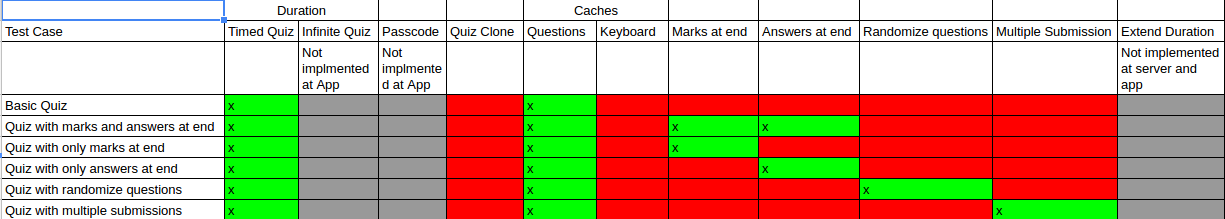
\includegraphics[scale=.4]{diagrams/test-matrix-1} 
\vspace{1cm}
\caption{Test Matrix of Different Quiz Settings}
\end{center}
\end{figure}


\begin{figure}[h!]
\begin{center}
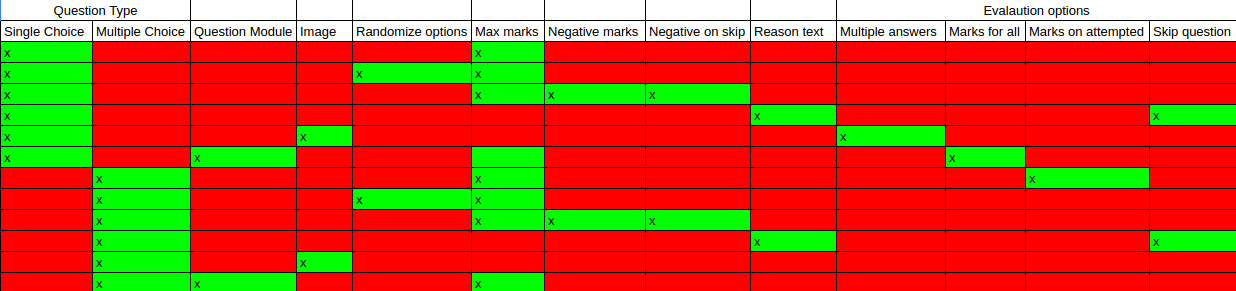
\includegraphics[scale=.4]{diagrams/test-matrix-2} 
\vspace{1cm}
\caption{Test Matrix of Question Types}
\end{center}
\end{figure}